\section{The \texorpdfstring{\Gls{imacs}}{IMACS} framework}\label{lkas_hil}
We consider a motivating case study of a \gls{lkas} to demonstrate our approximation-aware \gls{ibc} design approach.
The \gls{imacs} framework helps to test and evaluate the impact of approximation in closed-loop feedback systems.
First, the resilience of the given \gls{ibc} system to different approximation choices is analysed. Second, for each approximation choice, the sensing delay is computed, and the error due to approximations is quantified using the \gls{imacs} framework.
Then, an approximation-aware controller is designed, for each approximation choice, by considering the sensing delay and modelling the quantified error due to approximations as sensor noise (explained later in Section \ref{lqg_control}).

Fig.\ \ref{fig:hilsetup} illustrates the \gls{imacs} \gls{hil} simulation setup for \gls{lkas}. 
The detailed description of the \gls{imacs} framework is reported in~\cite{mohamed2019imacs}. The \gls{imacs} framework supports \gls{xil} simulation and is not just limited to \gls{hil} simulation.
It simulates a vehicle with a top look ahead camera using a physics simulator engine, e.g.. Webots~\cite{michel2004cyberbotics}, and interacts with a hardware platform, e.g.. an NVIDIA AGX Xavier platform, using the \gls{tcpip} protocol. The simulator works in a server-client configuration, wherein the physics simulator engine acts as the server while the platform acts as the client. The server (Webots) progresses simulation in full synchronization with the client (NVIDIA AGX Xavier) \cite{nvidiaAGX}. At each simulation step, the camera sensor simulated in Webots generates a raw image containing state information $x[k]$, that is fed to the NVIDIA platform. It executes the sensing (\taskS) and control (\taskC) tasks to generate control input $u[k]$, which is communicated back to Webots for actuation. After actuation, the simulation progresses to the next step. 

% \vspace{-5 pt}
\begin{figure}[t]
	\centering
	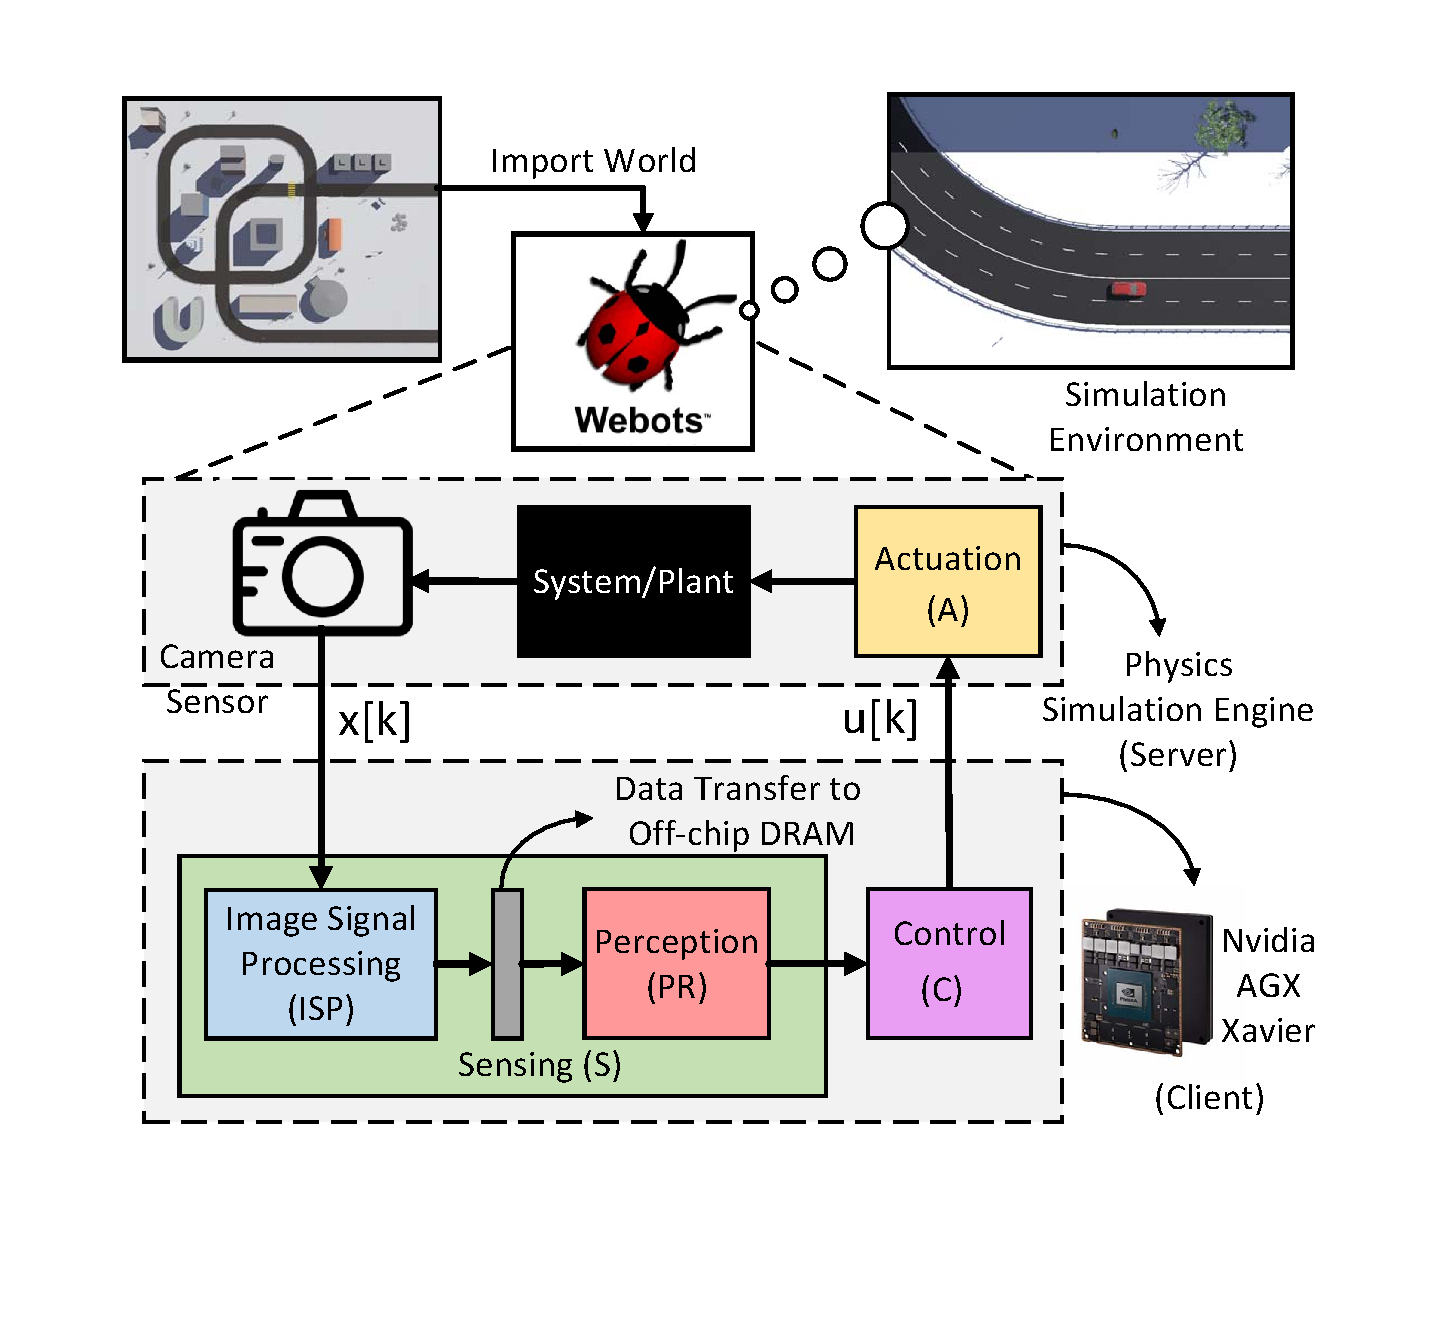
\includegraphics[width= 0.8\textwidth]{figs/lkas_block.pdf}
	\caption{{\Gls{imacs} \gls{hil} simulation setup for the \gls{lkas} system.}}
	\label{fig:hilsetup}
% 	\vspace{-5pt}
\end{figure}

For the scope of this chapter, the \gls{imacs} framework uses the following configuration settings.
The camera sensor in the Webots simulator is modelled based on the AR1335 \gls{cmos} digital image sensor \cite{camsensor} and is set to a resolution of 720p\footnote{We observe that state-of-the-art lane detection algorithms \cite{NvidiaLanenet} operate on low-resolution images. So, we perform our evaluation using downscaled (512$\times$256) sensor images. We believe our approach is also effective for high-res images required in applications like object detection.}. The camera frame rate is varied between 30~fps, 60~fps and 120~fps, depending on the sampling period of the controller. The actuation dynamics are modelled based on \cite{RandyFrank2016}. The vehicle is initially positioned with a fixed bias of 15~cm from the lane centre to test the control performance. A lane width of 3.25~m is considered, as per standard road safety guidelines. The Webots simulation step is set to 1~ms, while the vehicle speed $v_x$ is set to 50~km/hr for all of our evaluations.

\begin{figure}[t]
    \centering
    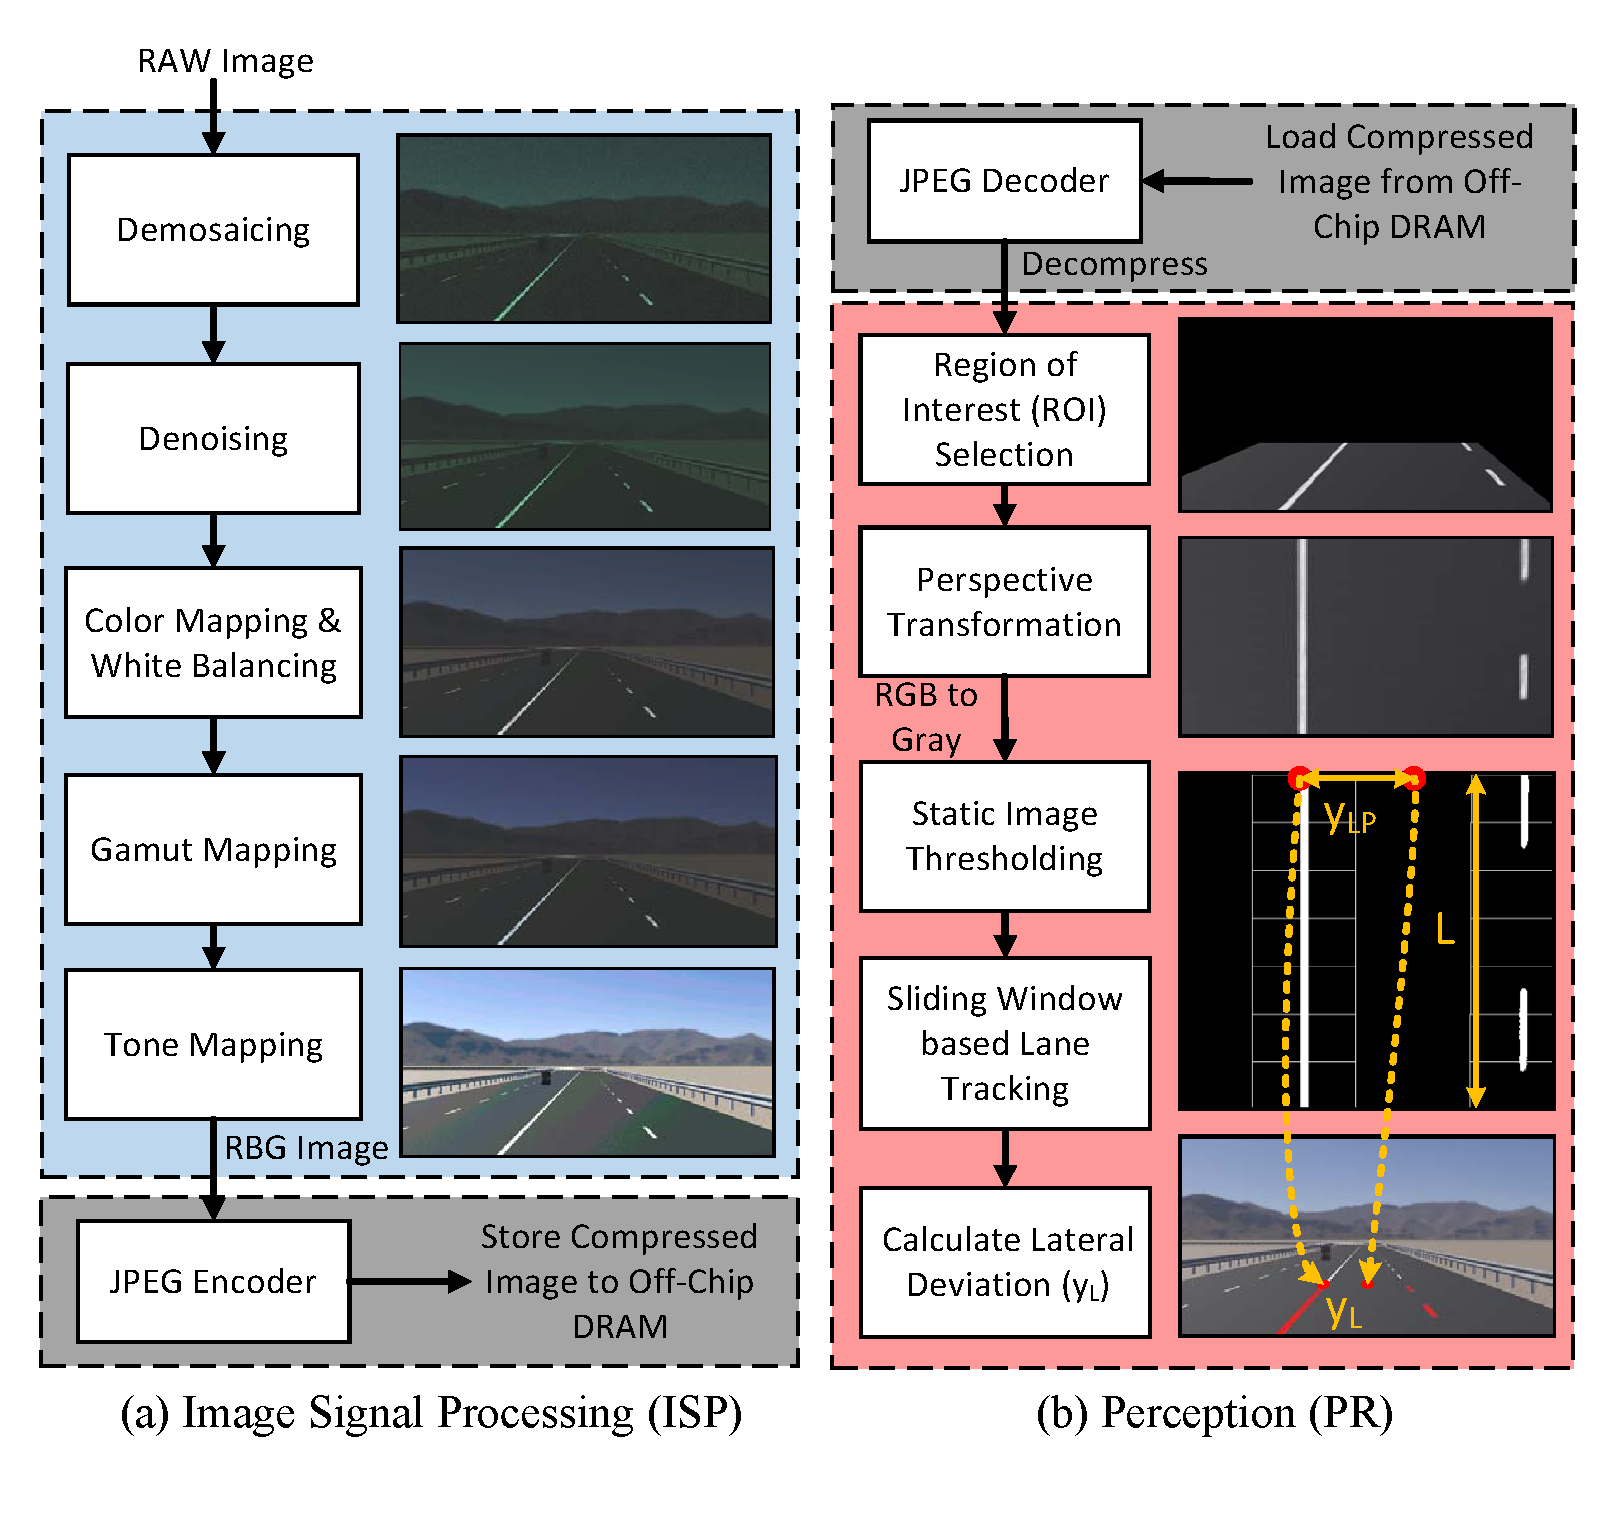
\includegraphics[width= 0.8\textwidth]{figs/isp_per.pdf}
    \caption{{Overview of \gls{isp} and \gls{pr} stages with their corresponding outputs.}}
    \label{fig:isp}
    % \vspace{-10 pt}
\end{figure}

\section{\texorpdfstring{\Gls{lkas}}{LKAS} implementation: overview}\label{lkas_algo}
A \gls{lkas} consists of six main components/stages: Camera Sensor, \gls{isp}, data compression, \gls{pr}, control (\taskC) and actuate (\taskA), as shown in Fig.\ \ref{fig:hilsetup}. The camera sensor and actuation are modelled and executed in Webots. \gls{isp}, data compression, \gls{pr} and control are executed on the NVIDIA AGX Xavier platform. Below, we provide an overview of these stages. The \gls{isp} and \gls{pr} stages are also illustrated in Fig.\ \ref{fig:isp}.

\noindent
\subsection{\Acrfull{isp} and \acrfull{pr}}
\par An \gls{isp} pipeline transforms a RAW image in the Bayer domain to pixels in the RGB domain through a series of image enhancing stages. Modern \glspl{isp} comprise of hundreds of proprietary stages. However, in this work, we consider a set of five essential stages common to all \gls{isp} pipelines, demosaic, denoise, color map, gamut map and tone map, as defined in \cite{buckler}. Fig. \ref{fig:isp}(a) shows these five stages along with their corresponding outputs. It is worth noting that the RGB output from the \gls{isp} pipeline is typically stored in the main memory (off-chip \gls{dram}) due to the large size of the image data. In this work, we consider JPEG compression (see Fig. \ref{fig:isp}) to reduce the data communication between different processing stages like \gls{isp}, \gls{pr}, etc.  

\par The \acrfull{pr} stage calculates the lateral deviation of the vehicle from the centre of the lane by performing preprocessing, feature extraction and inference steps on the decompressed \gls{isp} output.
During \textit{preprocessing}, first, the \gls{roi} is selected based on the scene. A perspective transform is then performed on the \gls{roi} to get a bird's eye view of the lane ahead (see Fig.\ \ref{fig:isp}~(b) block 2 of the PR stage). During \textit{feature extraction},  the candidate lane pixels are extracted from the bird's eye view image. For this, the bird's eye view image is converted to grayscale, and subjected to binarization using static thresholding (see Fig.\ \ref{fig:isp}~(b) block 3 of PR). Finally, candidate lane pixels are obtained using sliding windows ranging from bottom to top of the image. During \textit{inference}, 
first, the previously identified lane positions markers are fit to a second-order polynomial. Then, these polynomials are used to calculate the centre of the lane at a look-ahead (L) distance. The centre of the image in the x-direction is considered as the vehicle's current position. Using these two metrics, the lateral deviation in the transformed domain ($y_{LP}$) is calculated (see Fig.\ \ref{fig:isp} (b)). A reverse perspective transform gives the final lateral deviation ($\yL$) (see Fig.\ \ref{fig:isp}~(b))

\noindent
\subsection{Discrete-time control implementation (\taskC)}
\label{sec:ch6_lqr}
We consider the bicycle model introduced in Section~\ref{sec:lkas_case_Study} for simulating the \gls{lkas} and it is described as follows,
\begin{align}
     \dot x(t) &= \Acont x(t) + \Bcont u(t), \nonumber
     \\
     y(t) &= \Ccont x(t), \nonumber
\end{align}
where the following vehicle parameters in Section~\ref{sec:lkas_case_Study} are adapted for the BMWX5 car model in Webots (which are parameters of system matrices $\Acont$, $\Bcont$ and $\Ccont$):
$l_{f}$,\ $l_{r}$ ($=1.6975$ and $1.2975$ m respectively) denote distance of the front and rear axles from the \gls{cog};
$I_{\psi}$ ($=6337.74$ kg$\cdot$m$^2$) is the total inertia of the vehicle around its \gls{cog};
$c_{f}$,\ $c_{r}$ (${=2\times60000\text{~N/rad)}}$ denote cornering stiffness of the front and rear tires; and the total vehicle mass is $m$ ($=2000$ kg).

As in earlier chapters, we guarantee constant sensing-to-actuation delay $\tau$ by enforcing an implementation with time-triggered activation of tasks.
An implementation is annotated with a pair $(h_i,\tau_i)$ that models the sampling period and delay associated with it.
The \gls{zoh} method is used to discretize the system~\cite{franklin1998digital} with the annotated $(h_i,\tau_i)$ to obtain an augmented system of the form:
\begin{math}
z[k+1]= \Adyn z[k] + \Bdyn u[k],
\end{math}
where $\Adyn$ and $\Bdyn$ are discretized matrices and the augmented system states $z[k]=\left[x[k]\ \ u[k-1]\right]^T$.

\noindent\textbf{Control law:} The control input $u[k]$ is a state feedback controller of the form 
 \begin{align}
		u[k] = \Kgain z[k], 
		\nonumber
		%\label{eqn:u[k]}
 \end{align}
 where $\Kgain$ is the state feedback gain.  
 We design $\Kgain$ using the optimal \gls{lqr}~\cite{franklin1998digital}.
 The control objective is for the output $y[k]\rightarrow 0$, when $k\rightarrow\infty$.

\subsection{Hardware support for \gls{lkas}}\label{lkas_hw}
An industrial embedded heterogeneous platform NVIDIA AGX Xavier \cite{nvidiaAGX} is considered for \gls{lkas} implementation, as explained in Section~\ref{sec:nvidia_agx} and illustrated in Fig.\ \ref{fig:platform}~(a). 
Note that Fig.\ \ref{fig:platform}~(a) only shows the IPs used in this work. 

%\vspace{-5 pt}
\begin{figure}[ht]
    \centering
    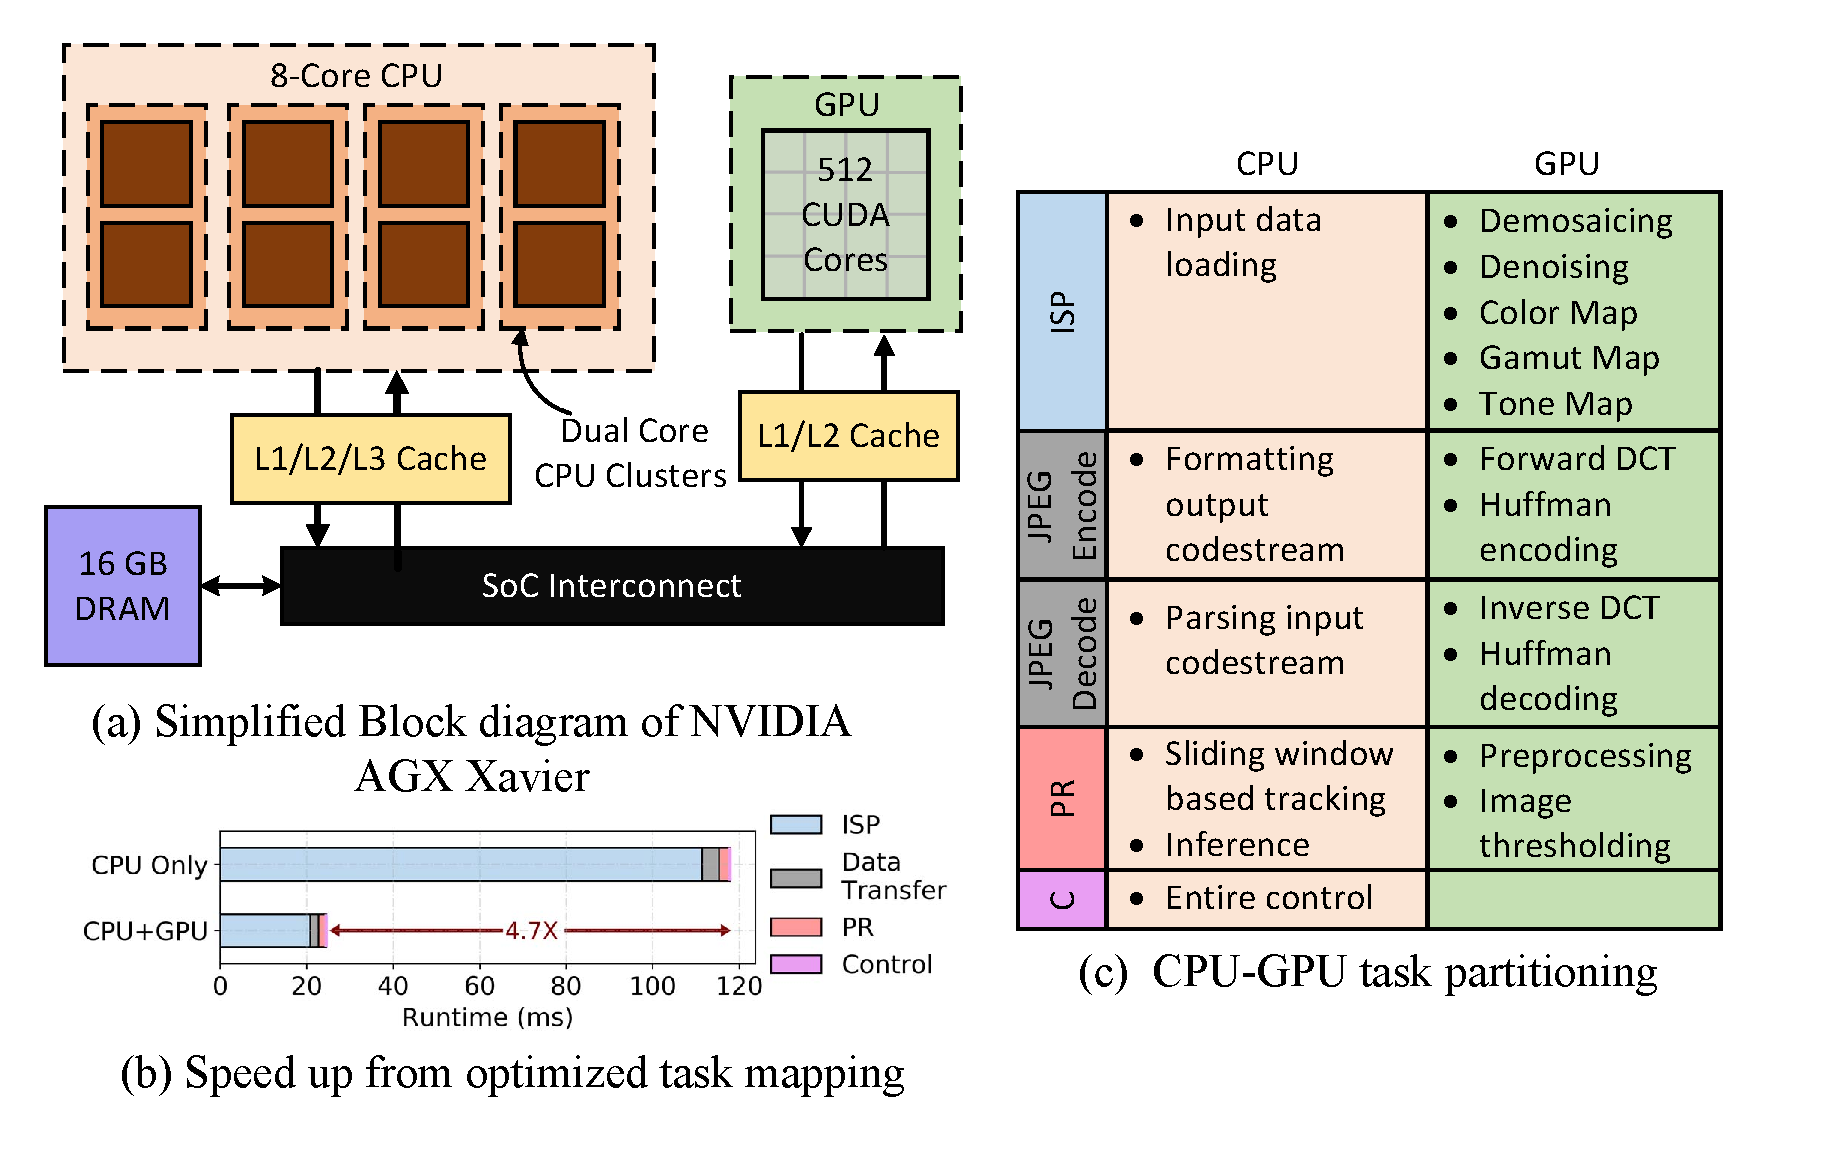
\includegraphics[width= \textwidth]{figs/lkas_hw_overview.pdf}
    %\vspace{-15pt}
    \caption{{\gls{lkas} task mappings on an 8-core \gls{cpu}+\gls{gpu} default configuration (\gls{cpu}\_8C+\gls{gpu}). A comparison with software only (8-core \gls{cpu}) configuration is shown. Runtimes are shown for image workloads of (512x256) resolution.}}
    \label{fig:platform}
    %\vspace{-5 pt}
\end{figure}

\par \noindent \textbf{Baseline Task Mapping: } The main tasks in the \gls{lkas}  that are executed on the NVIDIA platform are \gls{isp}, JPEG encode/decode, \gls{pr} and control (\taskC). As an initial step, we map all the tasks to an 8-core \gls{cpu} only configuration. The measured runtimes of the individual tasks are shown in Fig.\ \ref{fig:platform}(b). The \gls{isp} takes most of the computation time. So, we map all the \gls{isp} tasks to the \gls{gpu} (see Fig.\ \ref{fig:platform}~(c)). The \gls{isp} is optimized using Halide \cite{halide} domain-specific language with \gls{gpu} as backend. Additionally, we also map parts of the JPEG encoding/decoding and \gls{pr} to the \gls{gpu}. Fig.\ \ref{fig:platform}~(c) gives a detailed mapping overview. Task offloading from \gls{cpu} memory to \gls{gpu} memory is a major bottleneck. We make use of the unified memory (a single memory address space accessible from any processor in a system) support in NVIDIA Volta \glspl{gpu} to optimize our mappings further. The control task \taskC\ is light in compute, so we map it to the \gls{cpu}. This CPU-GPU task mapping gives a runtime speedup of 4.7$\times$ over the initial 8-core \gls{cpu} only mapping (see Fig.\ \ref{fig:platform}~(b)). \textit{We consider this as a baseline for exploring approximation opportunities in \gls{lkas}}.